\chapter{Natural Language Processing}
\label{chap:nlp}

It is often challenging to realize the complexity behind \glsfirst{nl}, even to experts. First of all, Language is an academic field of study, implying multi-disciplinary skills. And secondly, staying up to date with evergrowing tools and new \gls{sota} algorithms proves to be challenging. \gls{nl} is the fundamental communication element for humans, \gls{nlp} is the field of \gls{ml} studying \gls{nl} with the goal of providing the ability to machines to handle and mimic \gls{nl} to create human-like verbal interactions. Beyond words and grammar rules, \gls{nl} is a complex orchestration of subtleties, intuitively handled by humans, but not for easily handled by machines. Nonetheless, \glspl{nlp} technologies are massively used in our daily lives, including information extraction, summarization, and conversation simulation. However, even if machines are given the same language rules as humans, they do not yet understand the manipulation they are processing, as humans would do. Indeed, \gls{nlp} algorithms are applying pre-defined or multiple examples-based learned rules, which may result in ambiguities while applying \gls{nl}. Using a rule-based approach \ref{chatbot:rulebased} to build a \gls{nl} model would result into near to infinite amount of conditions, this is the main reason for \gls{nlp} to be particularly present \gls{ml}, particularly in \gls{dl}. 


%\section{\acrlong{nlp} Technologies}
\section{Word Embeddings}
\label{nlp:we}
Commonly used as the first data pre-processing in \gls{dl} \gls{nlp}. Those \glsfirst{ul} algorithms capture syntactical and semantical words representation from large unlabelled corpora datasets as vectors by building a multi-dimensional matrix. On average, dimensions are held in a scope of 100 to 400, and thanks to its the vectorized nature captured words, geometrical operations can be applied, such as the cosine functions to calculate word similarities. Another feature related to word embeddings, is the ability to apply analogical operations such as \textit{'king' - 'man' + 'woman' = 'queen'}, which popularize Word2Vec \ref{nlp:word2vec} and gave credits to the method, even if the justification to this effect has been theorietized 4 years later \footnote{Skip-Gram - Zipf + Uniform = Vector Additivity \autocite{paper:gittens-etal-2017-skip}} by stating that the compositionality is only seen when assumptions are held, in particular when words are uniformly distributed in the embedding space.

\subsection{Word2Vec and GloVe}
\label{nlp:word2vec}
Published by \textit{Google} in 2013, Word2Vec \autocite{paper:word2vec}, and its competitor GloVe \autocite{paper:glove} published by the \textit{University of Standford} in 2014, both use a \gls{snn}, as illustrated on Figure ~\ref{fig:fig_snn}, similarly to \gls{sl} by feeding as input a text corpora, and outputting word vectors with a given vocabulary. Training and testing is straightforward but painful tweaking make it hard to build good generalized word embedding representations. Even if the \gls{snn} could remind a \gls{dl} approach, it is only has one hidden layer; however, the output word vectors are particularly useful for \gls{dnn} as input.

\begin{figure}[H]
    \centering
    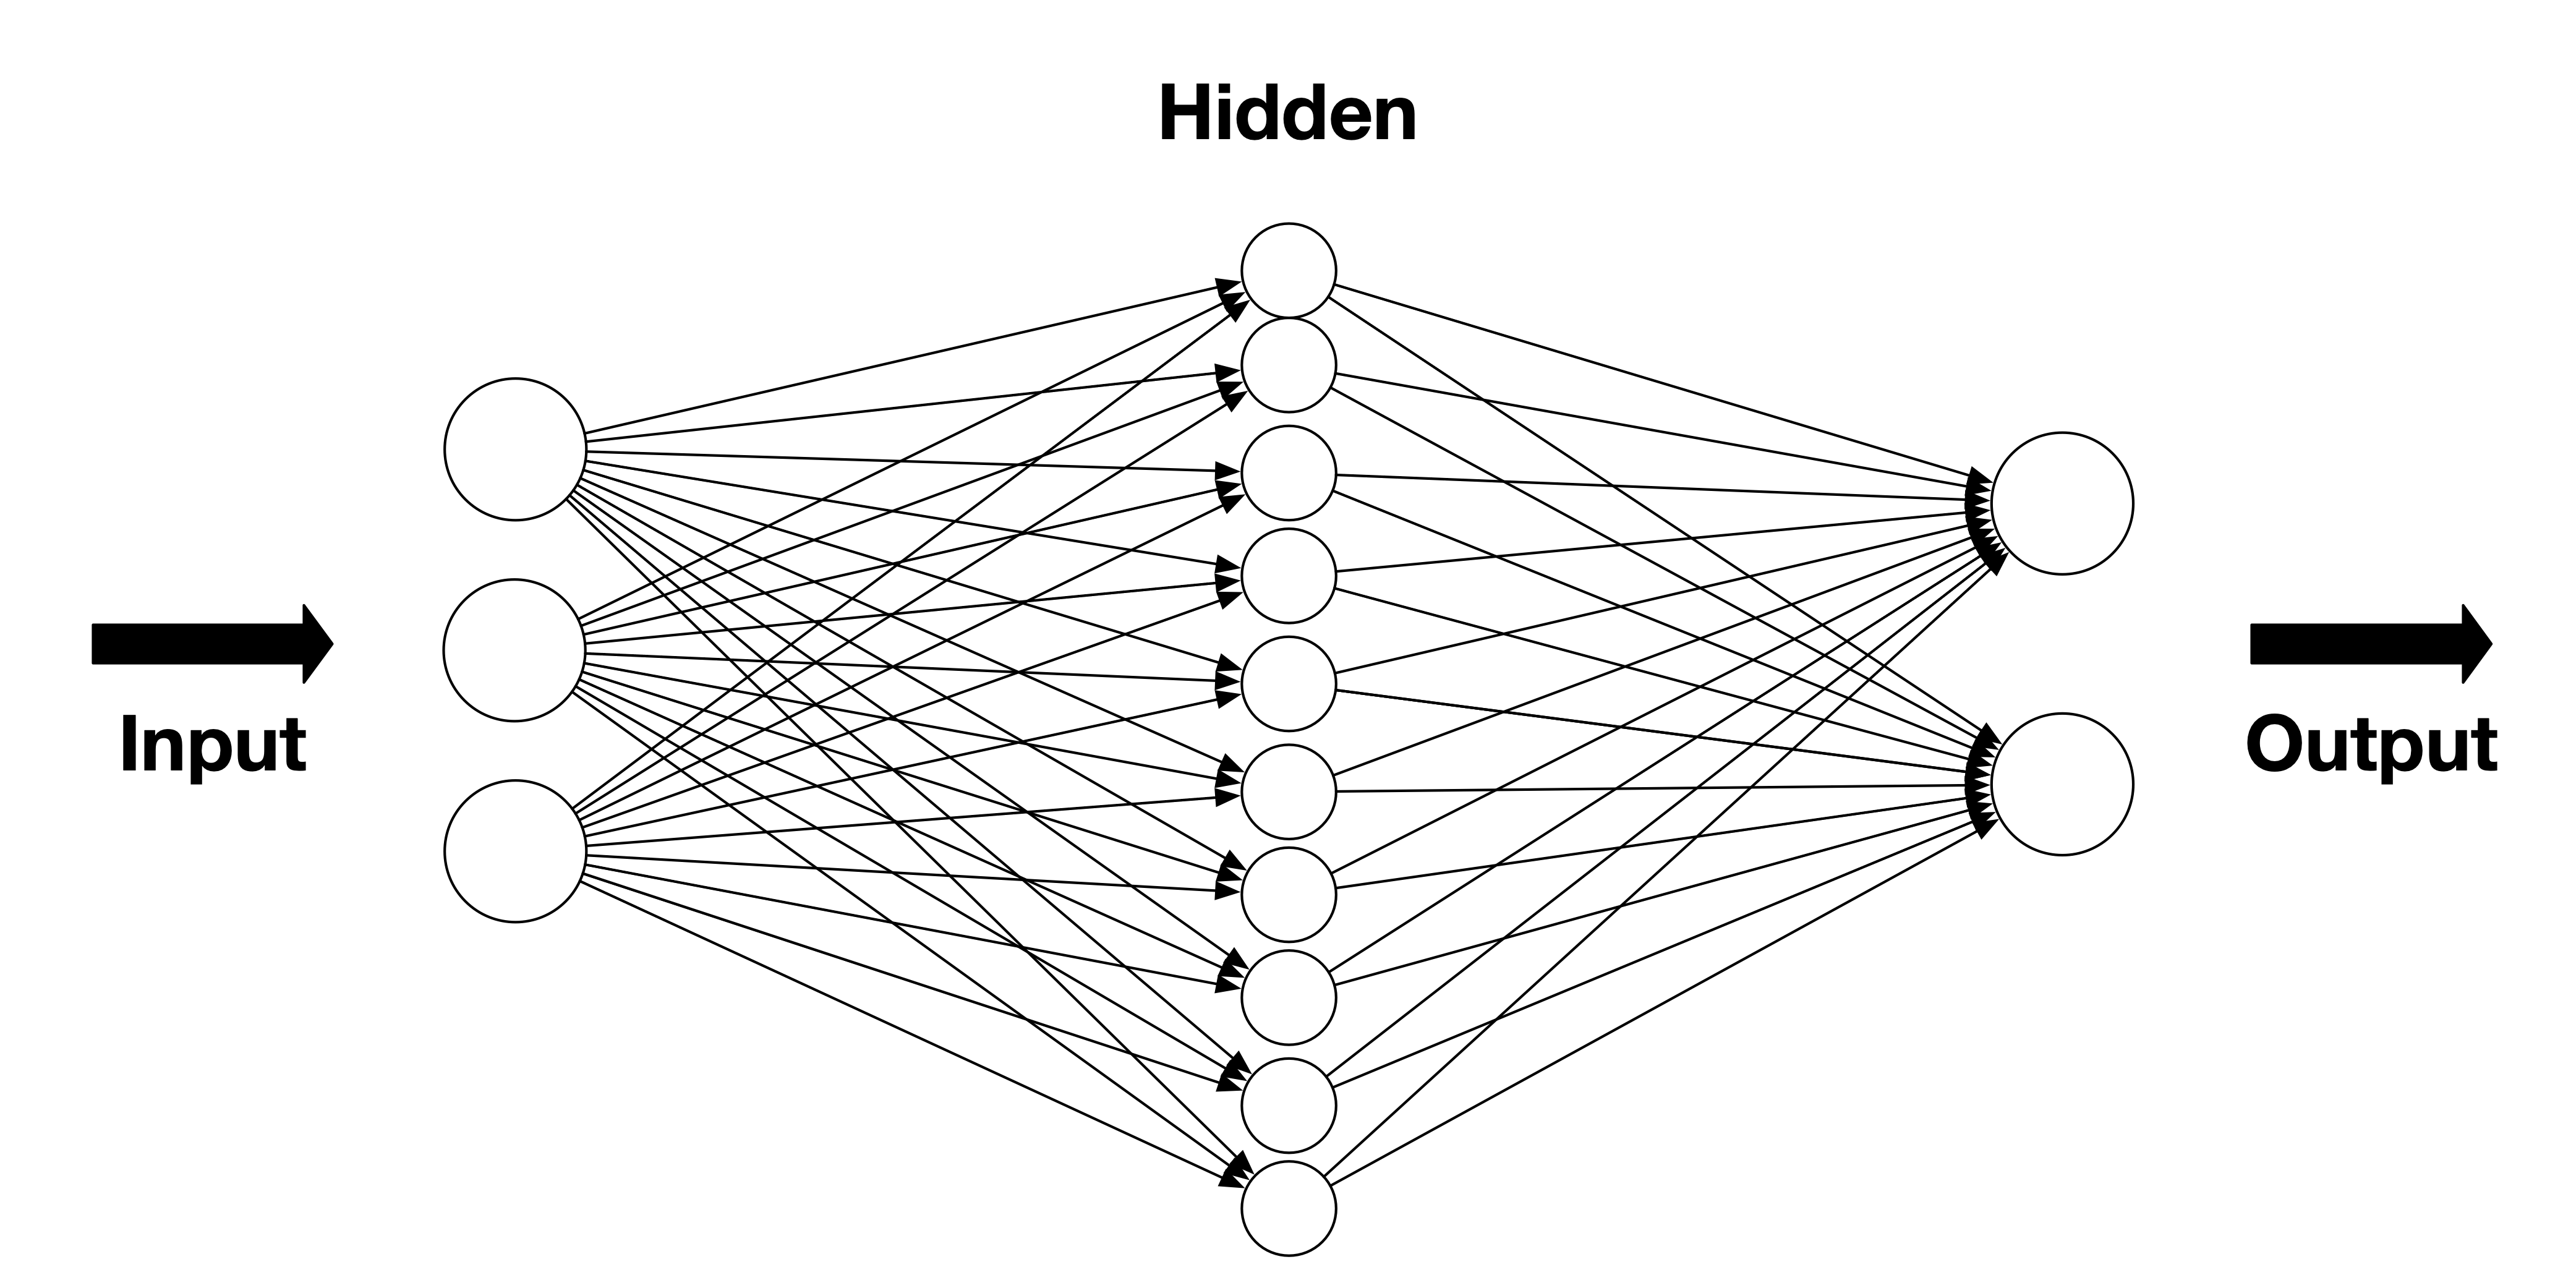
\includegraphics[width=\textwidth,keepaspectratio=true]{fig_snn}
    \caption{Illustrative representation of a Shallow Neural Network}
    \label{fig:fig_snn}
\end{figure}

\subsection{Out of Vocabulary Problem}
\label{nlp:oov}
A common issue in \gls{we} is related to the vocabulary itself when words are unknown, called the \gls{oov} issue. The issue occurs when post-training the model is requested to provide a vector representation that it never seen before. A solution could be to handle the exception by forwarding it to a default or pre-defined error vectors such as a series of zeros. We could approach the problem sophisticatedly, by defining on-the-fly \gls{oov} words with at a high learning rate as the sum of word-vectors contextualizing the \gls{oov}  \autocite{paper:journals/corr/HerbelotB17}. Another solution would be to fallback to \ref{nlp:ce} by either training a model to compositional map characters to words \autocite{paper:journals/corr/PinterGE17}, or using \gls{ce} as a whole instead of \gls{we} \ref{nlp:ce}.

\section{Character Embeddings}
\label{nlp:ce}
Additionally to \gls{we} similar abilities to capture semantics and syntactic relations, \gls{ce} handles by design \gls{oov} issues \ref{nlp:oov}, which is common for rich vocabularies languages. Instead of using words as vocabulary, \gls{ce} uses individual characters and semantics embeds words using the characters compositionally, which avoids word segmentation and makes it useful for language such as Chinese \autocite{paper:conf/ijcai/ChenXLSL15}. Moreover, \gls{ce} can also perform complementary \gls{nlp} tasks such as \gls{pos-tag} \autocite{paper:conf/icml/SantosZ14}, \gls{ner} \autocite{paper:ma-etal-2016-label}, Sentiment Analysis \autocite{paper:2017HaoYetal} and \gls{lm} \autocite{paper:journals/corr/KimJSR15}. As it is at the time of writing, \textit{FastText} based on the a morphologically-rich skip-gram approach \autocite{paper:journals/corr/BojanowskiGJM16} as been popularilized due to its ability to be scalabely trained on large corpora fast, and effectively. 


\section{Pre-trained Language Models}
\label{nlp-lm}
Beyond complex semantics and syntaxes provided by \gls{we} \ref{nlp:we} and \gls{ce} \ref{nlp:ce}, \glspl{lm} handles \gls{cwe} by additionally capturing the polysemy across multiple contexts. Indeed, it was discovered that a distributed semantic, such as \gls{we} and \gls{ce} are not sufficient to infer context within the embeddings \autocite{paper:journals/corr/LucyG17}. A solution is to combine overall word representations from \gls{we} with \textit{ELMo} \autocite{paper:journals/corr/abs-1802-05365}, as its authors suggests, a \gls{bilm} able to build deep contextual word embeddings by handling multiple word representations. As mentioned in the study, handling polymesy is just one of the \glspl{lm} features as they are theoritized to capture meaningful \gls{nl} traits used in \gls{nlu} and \gls{nlg}. To increase the \gls{lm} quality, defined by language syntactic and semantical complexities captured, \gls{ul} on large corpora is popularly used, as no labeled data is required.


\section{Transformers}
\label{nlp:transformers}
Since 2017 \autocite{paper:journals/corr/VaswaniSPUJGKP17}, transformer are defining the \gls{sota} for multiple \gls{nlp} tasks with its parallelized attention \ref{nlp:attention} architecture, multi-directional pre-trained \gls{lm} such as \gls{gpt2} or the \gls{bert} family, additionally to their ability to capture features at sentence level, out-performs by a large margin previously mentioned \gls{nlp} technics at tasks such as \gls{qa} by performing fine-tuning.


\subsection{Attention Mechanism}
\label{nlp:attention}
Introduced in 2014, The Attention Mechanism \autocite{paper:bahdanau2014neural} solved the problem raised by tasks such as text summarization, machine translation or sentiment analysis where the input could be too rich to perform a selective encoding. Originally, the last hidden state of the decoder is used by a multi-layer perceptron to define the attention from an input hidden state. The mechanism even got adapted from \gls{nlp} to Computer Vision and shown its ability to replace \gls{cnn} with \gls{sota} results \autocite{paper:journals/corr/abs-1906-05909}.

\subsection{The architecture}
Even if Transformers \ref{fig:fig_external_transformer_1} are using an encoder and decoder similarly to \gls{rnn} and \gls{cnn}, the overall architecture focuses mainly on the attention mechanism to capture the relation between the input and the output, making it well parallelizable and less time consuming during training. Additionally to the attention mechanism, transformers are also using techniques such as layer normalization, dropouts, and positional encodings.

\begin{figure}[H]
    \centering
    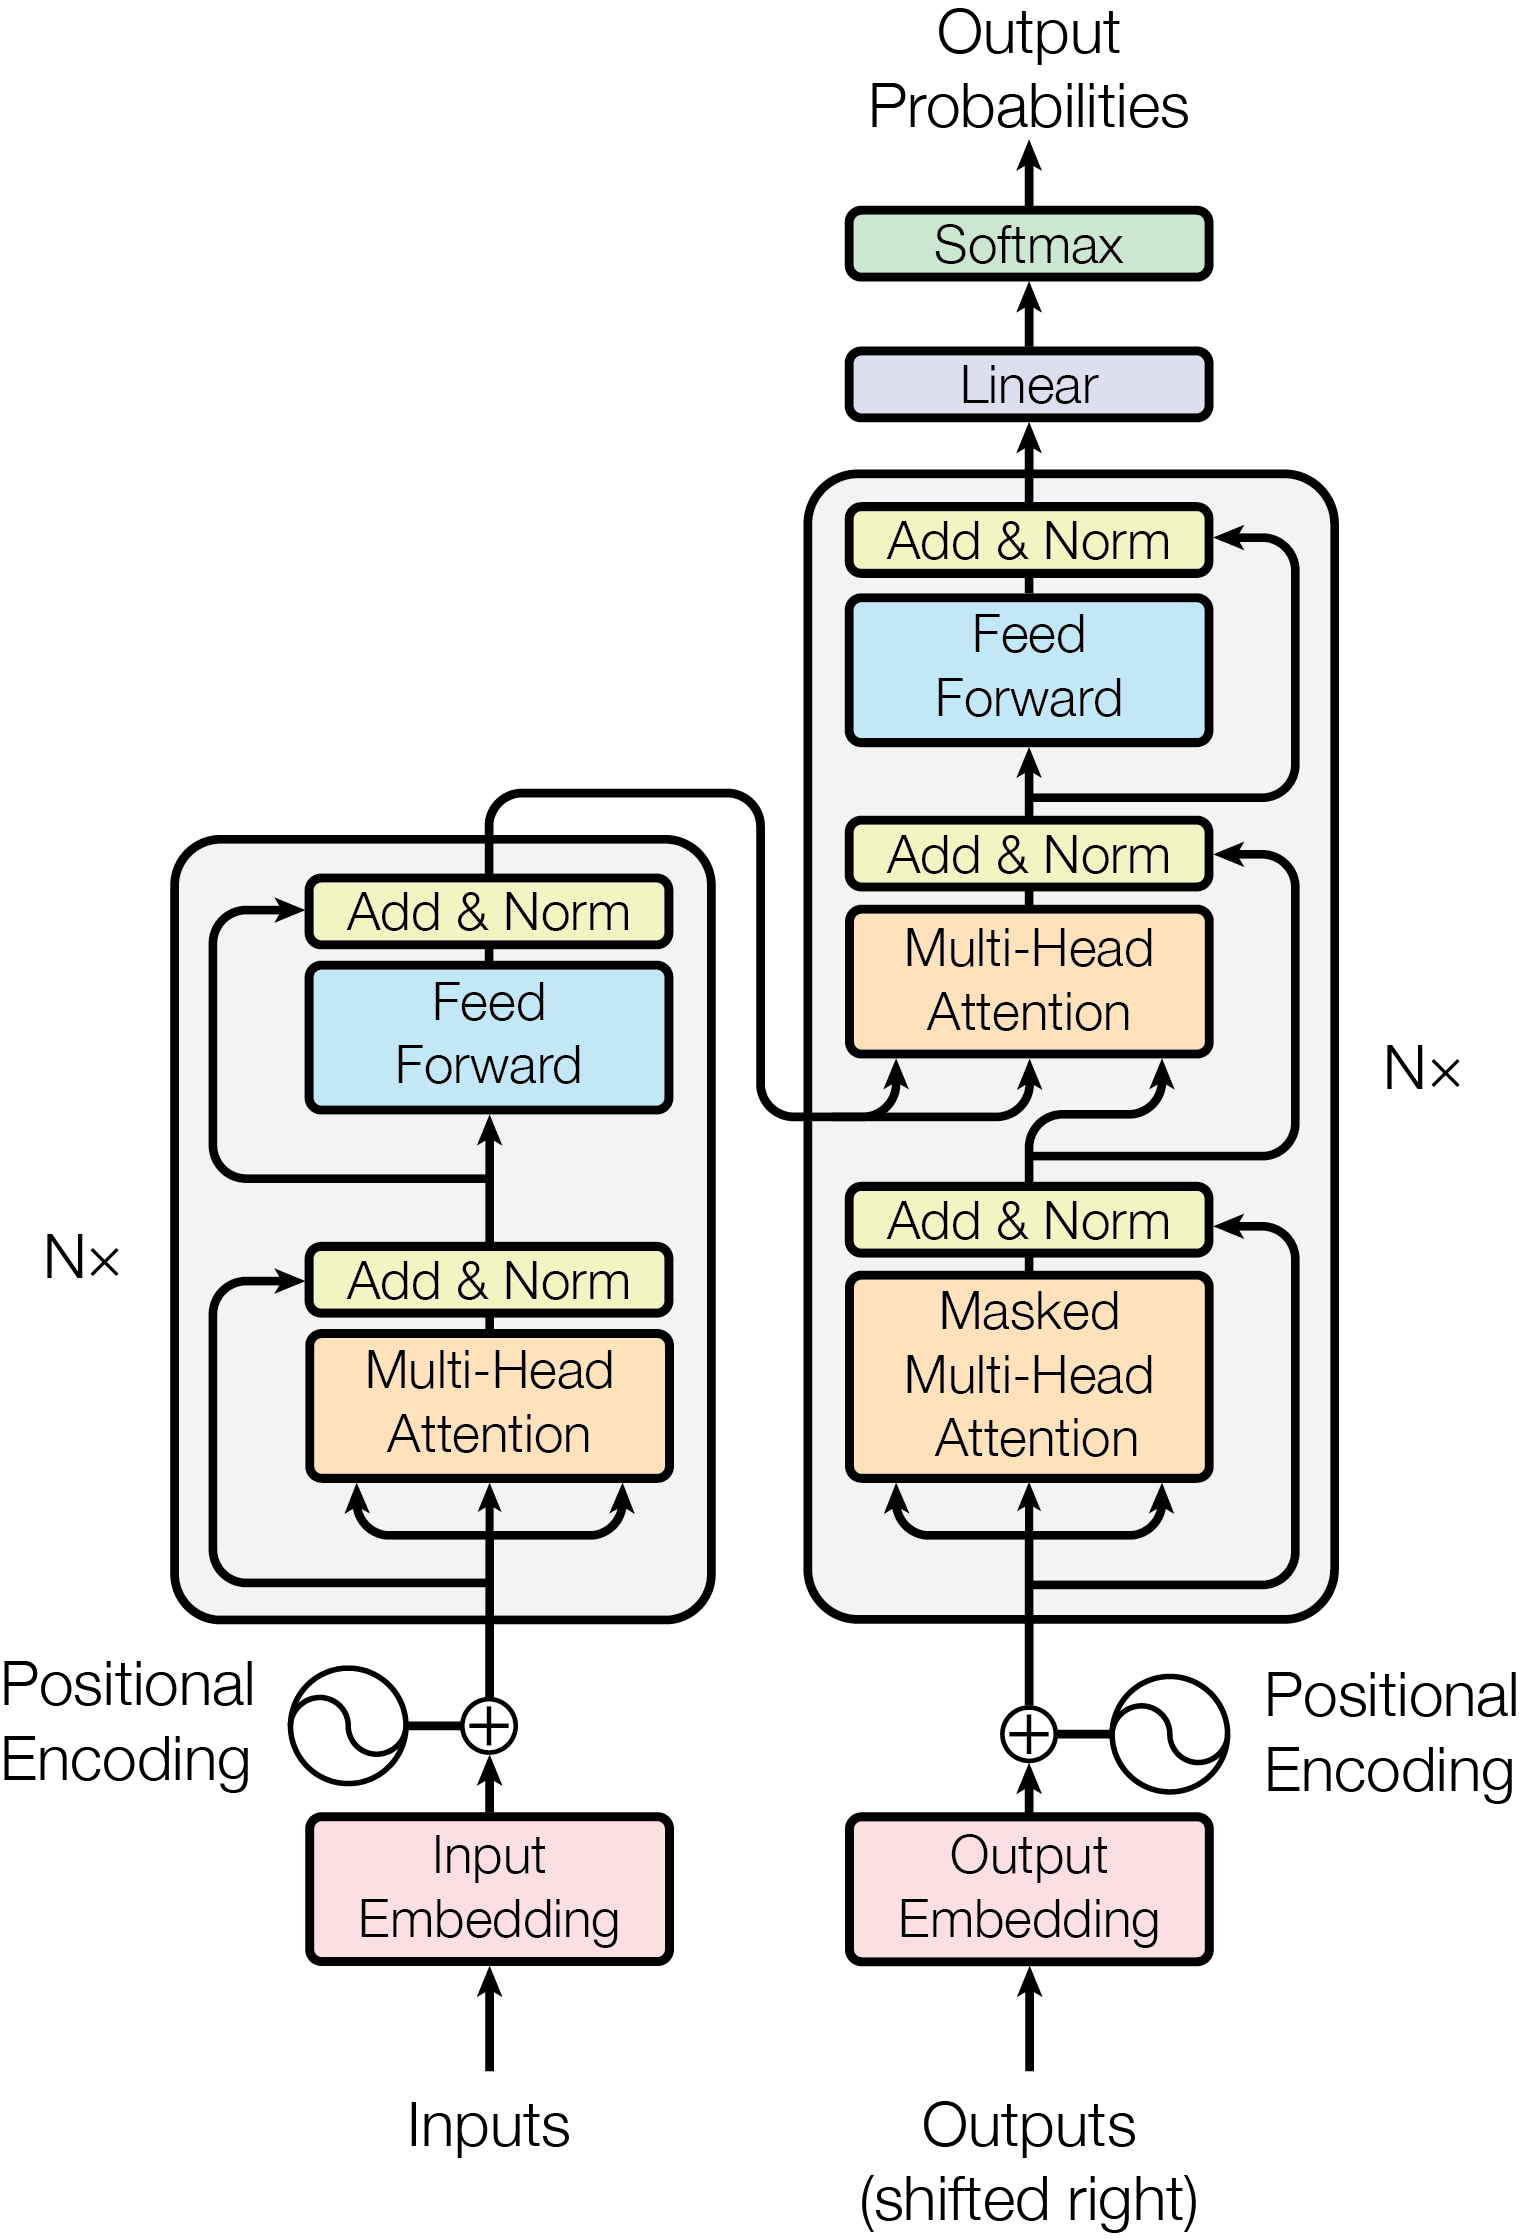
\includegraphics[width=\textwidth/2,keepaspectratio=true]{fig_external_transformer_1}
    \caption{Represents the Transformer architecture. Figure 1 from \autocite{paper:journals/corr/VaswaniSPUJGKP17}}
    \label{fig:fig_external_transformer_1}
\end{figure}



 To solve the sequential processing during encoding bottleneck from the Attention Mechanism \ref{nlp:attention}. The architecture discarded the usage of recurrence and convolutions and focuses on the attention mechanisms to capture the global relations between input and output.


\todo{The described approaches for contextual word embeddings promises better quality representations for words. The pre-trained deep language models also provide a headstart for downstream tasks in the form of transfer learning. This approach has been extremely popular in computer vision tasks. Whether there would be similar trends in the NLP community, where researchers and practitioners would prefer such models over traditional variants remains to be seen in the future.}

\subsection{Deep Learning}
\todo{What are the problems such as bias, and how it can accumulate? Used to predict the next step. Various techniques, such as generative, recursive, etc.}

\subsection{Unsupervised Deep Learning}
\todo{How and when unsupervised training is helpful for NLP. What are the techniques. Talk about fine tuning and re-training.}

\subsection{Generative Deep Learning}
\todo{Talk about the Variational Autoencoders and how they work. What are the problems to generate realistic sentences? Talk about the latest work made with VAE (2017?) and what is the outcome. Obviously talking about the Generative Adversarial Networks, and how they work. Talk about how to evaluate the generated outputs (with an oracle?) or with BLEU scores.}


\section{Honorable Mentions}

Even if Transformers has discarded CNN and RNN with the \gls{enc-dec} To solve the sequential processing during encoding bottleneck from the Attention Mechanism \ref{nlp:attention}. The architecture discarded the usage of recurrence and convolutions and focuses on the attention mechanisms to capture the global relations between input and output.

\subsection{Convolutional Neural Networks}
\todo{Explain what is a CNN, and how it is commonly used in sentence modeling. Say what the problems are. Compare with the Window Approach, which is working with the neighboring words. Talk about what is a Dynamic CNN and how DCNN can solve problems from CNN. Say that in the field of QA, the Multi-Column CNN \autocite{paper:Dong2015} approach is working on multiple aspects of a question to create a representation, which is working with Freebase (ancestor of wikidata and the knowledge graphs). Furthermore, in 2016, Severyn and Moschitti \autocite{paper:Severyn2016} proposed a QA model for Question and Answer sentences, which proposes to handle a form of relational information by matching words between question and answer pairs. Talk about the 2015 Dynamic Multi-Polling CNN \autocite{paper:Chen2015}, which incorporates events that trigger information for the polling layer. Talk about the Conditional Random Field. Explain the Time-delayed Neural Network. Conclude that CNNs, are good at mining semantics, however, they are very heavy models, plus they are not good are modeling long-distance information from a context point of view, which is a problem also for keeping a sequential order.}

\subsection{Recurrent Neural Networks}
\todo{Explain what is an RNN, basic, long short-term memory, gated recurrent units.  RNN over CNN have a memory from previous computation and take advantage of it. Based on \autocite{paper:Yin2017} say that there is no clear winner between RNN over CNN in NLP in performance, it depends on the global semantics and the task itself. Say that it's widely used in NLP tasks such as Language Modelling, Word and Sentence Classification, Machine Translation, Text generation, Image Captioning, Speech Recognition, and probably more. Say how it is useful in the previously named applications. Talk about the attention mechanism \autocite{paper:Bahdanau2014} and its parallelized version: The Transformer \autocite{paper:Vaswani2017}}


\subsection{Memory Networks}
\todo{Compare with the hidden vectors from encoders and decoders used in the attention mechanism, where here the hidden vectors are the input of the model. Talk about the Dynamic Memory Networks and how it is used in QA, POS, sentiment analysis, visual signals and probably more.}



\section{Common Natural Language Processing Features}
Most of the following technics have been introduced to \gls{nlp} by the \glsfirst{ir} field. Indeed

\begin{itemize}
    \setlength\itemsep{0em}
    \item \gls{tf-idf}: Used to set the word importance in corpora.
    \item \gls{cbow} [\ref{analyse:cbow}]: Counts the words occurrences throughout in corpus.
    \item Skip-Grams [\ref{analyse:skip-grams}]: Counts the occurrences of the character throughout in corpus.
    \item Topic modeling: Text clustering providing meaningful information to discover hidden structures via text chunking to identify the parts of the sentence in relation to each other.
    \item Segmentation: Split corpus into predefined parts, such as: \textit{sentences, paragraphs, chapters, etc.}
    \item Tokenization: Split the sentences into words.
    \item Tagging: Based on a pre-made dictionary, it gives a new layer of meaning to the word, such as: \textit{verb, adverb, noun, people name, locations, number, etc.}
    \item Dictionary: Use of tokenized words to build a dictionary, which could contain the word occurrences.
    \item Stop Words: Ignoring words only used as liaisons, and not containing information, such as: \textit{and, or, etc.}
    \item Stemming: Uniformizing words to their root by removing the prefix and suffix, such as: \textit{remake and loveable}.
    \item Lemmatization: Replace the words to their base form, such as \textit{conjugated verb}.
\end{itemize}
